% file: tree-traversal-depth.tex

\documentclass{standalone}
\usepackage{tikz}
\usepackage{tikz-qtree}

\begin{document}
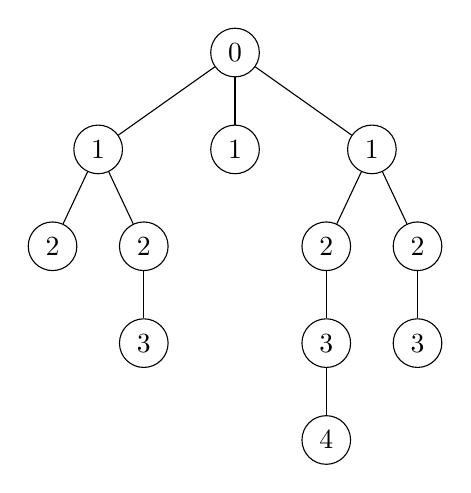
\begin{tikzpicture}[level distance = 35pt, sibling distance = 15pt,
  edge from parent/.style= { % added code
      draw, edge from parent path = {(\tikzparentnode) -- (\tikzchildnode)}}]
  \tikzset{every tree node/.style = 
    {align = center, circle, draw}}

    \Tree [.{0}	[.{1} [.{2} ]
		      [.{2} [.{3} ]]
                ]
		[.{1} ]
		[.{1} 
		  [.{2} 
		    [.{3} [.{4} ]] 
		  ] 
		  [.{2} 
		    [.{3} ] 
		  ]
		] 
	  ]
  \end{tikzpicture}
\end{document}

